\documentclass{beamer}
\usepackage[utf8]{inputenc}
\usepackage[russian]{babel}
\usepackage{caption}
\usetheme{Antibes}
\usecolortheme{seahorse}

\setbeamercovered{transparent}
\captionsetup[figure]{labelformat=empty,justification=centering}

\title[Введение в функциональное программирование]{Обзор курса}
\author{Олег Смирнов\\
\texttt{oleg.smirnov@gmail.com}}
\institute{УНК ``ИПСА'' НТУУ ``КПИ''}
\date{\today}
\begin{document}

\begin{frame}
\titlepage
\end{frame}

\begin{frame}{Программа на сегодня}
  \begin{itemize}
    \item Вводная лекция и обзор курса
    \item Первая лекция -- итеративные и рекурсивные процессы
  \end{itemize}
\end{frame}

\begin{frame}{Немного об авторе}
  \begin{itemize}
  \item {\bf 1999-2005:} Факультет прикладной математики КПИ
  \item {\bf 2003-2005:} x86 Asm, C; reverse engineering, системное программирование
  \item {\bf 2005-2009:} C++, Perl, Python; распределённые системы, сетевые протоколы
  \item {\bf 2009-2010:} Системы поддержки операций; курс алгоритмов в Global Logic
  \item {\bf 2011-сейчас:} Erlang, Ocaml; высоконагруженные системы, социальные сервисы
  \end{itemize}
\end{frame}

\begin{frame}{``Функциональщина'' глазами обычного программиста}
  \small{~~q~a~b~c~=~putStrLn~\$~b~++~[toEnum~10,~'q',~'(']~++~show~b~++\\
    ~~[',']~++~show~c~++~[',']~++~show~a~++~[')']\\
    ~~main~=~q~\char34 q~a~b~c~=~putStrLn~\$~b~++~[toEnum~10,'q','(']~++~show~b~\char34 ~++~\\
    ~~\char34 ++~[',']~++~show~c~++~[',']~++~show~a~++~[')']\char34 \\
    ~~\char34 def~q(a,b,c):print~b+chr(10)+'q('+repr(b)+','+repr(c)+','+repr(a)+')'\char34 \\
    ~~\char34 def~e(x)~return~34.chr+x+34.chr~end;def~q(a,b,c)~\char34 ~++~\\
    ~~\char34 print~b+10.chr+'main=q~'+e(b)+'~'+e(c)+'~'+e(a)+'~'+10.chr~end\char34}
\end{frame}

\begin{frame}{``Функциональщина'' глазами обычного программиста}
\begin{figure}
   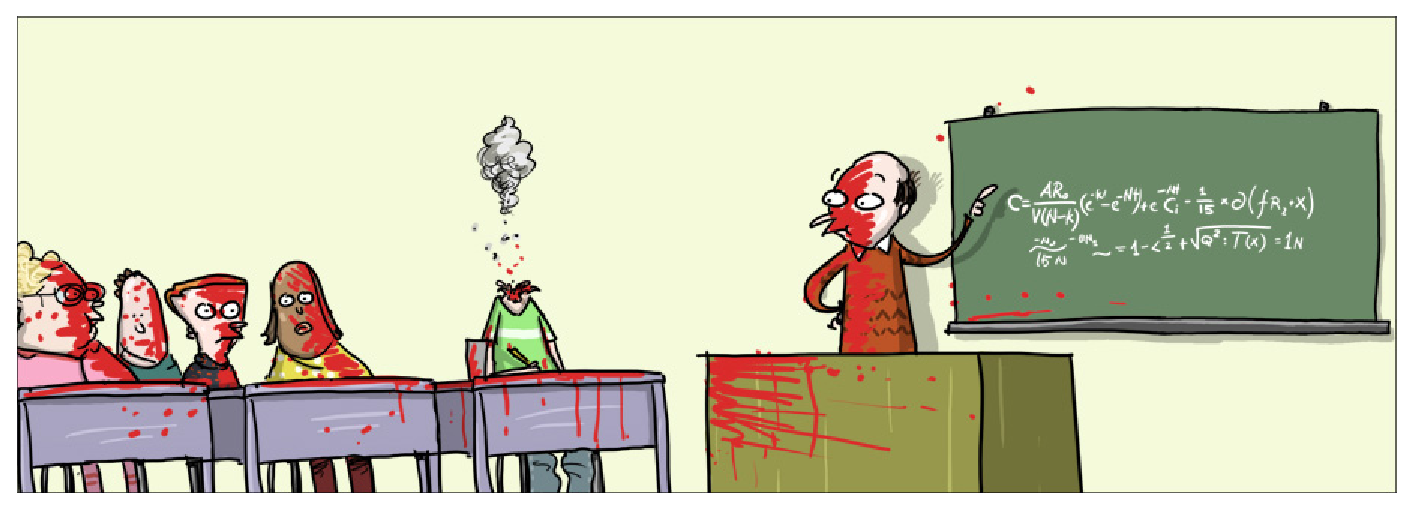
\includegraphics[scale=0.44]{lecture0/Matematik-Hjerne-Formel-WM_strip_DK_20090625.eps}
\end{figure}
\end{frame}

\begin{frame}{Цели курса}
  \begin{enumerate}
  \item Практика функционального программирования
  \end{enumerate}
\end{frame}

\begin{frame}{Практика функционального программирования}
  \begin{figure}
    
\includegraphics[height=15mm]{lecture0/Barcap-logo.eps}
    
\includegraphics[height=15mm]{lecture0/logo_grammarly.eps}
  \end{figure}
  \begin{figure}
    
\includegraphics[height=15mm]{lecture0/Massive_Solutions.eps}
    
\includegraphics[height=15mm]{lecture0/Socialabs.eps}
  \end{figure}
\end{frame}

\begin{frame}{Цели курса}
  \begin{enumerate}
  \item Практика функционального программирования
  \item Изучение новой парадигмы (а не языка)
  \end{enumerate}
\end{frame}

\begin{frame}{Изучение новой парадигмы}
  \begin{itemize}
  \item Верификация -- доказываем программы как теоремы\pause
  \item Параллелиризм -- технология Google MapReduce и Apache Hadoop\pause
  \item Неизменяемое состояние -- меньше ошибок, выше ``вкуриваемость'' кода
  \end{itemize}
\end{frame}

\begin{frame}{Цели курса}
  \begin{enumerate}
  \item Практика функционального программирования
  \item Изучение новой парадигмы (а не языка)
  \item Приёмы функционального программирования
  \end{enumerate}
\end{frame}

\begin{frame}{Приёмы функционального программирования}
  \begin{itemize}
  \item Сборка мусора: появилась в LISP (1958), стала мэйнстримом в 1995 (Java)\pause
  \item Замыкания: появились в Scheme (1975), стали мэйнстримом в 2000-х (C\#, JavaScript)\pause
  \item Ленивая обработка: появилась в Miranda (1985), стала мэйнстримом в 2000-е (LINQ)
  \end{itemize}
\end{frame}

\begin{frame}{Приёмы функционального программирования}
  \begin{itemize}
  \item Функции высшего порядка: появились в LISP, сейчас мэйнстрим везде кроме Java\pause
  \item Вывод типов: появился в ML (1979), стал мэйнстримом в 2007 (C\#, Scala, C++0x)
  \end{itemize}
\end{frame}

\begin{frame}{Программа курса: первый семестр}
  \begin{itemize}
    \item Язык F\#\pause
    \item Азы: рекурсия, функции высших порядков, замыкания, алгебраические типы данных\pause
    \item Практика: простые алгоритмы и структуры данных, парсинг\pause
    \item Параллельное программирование: свёртки, пробеги и технология MapReduce
  \end{itemize}
\end{frame}

\begin{frame}{Программа курса: второй семестр}
  \begin{itemize}
    \item Язык Haskell\pause
    \item Чисто функциональный структуры данных и персистентность\pause
    \item Программирование с монадами\pause
    \item Классы типов\pause
    \item Математические основы ФП и начало теории типов
  \end{itemize}
\end{frame}

\begin{frame}{Administrativia}
  \begin{itemize}
  \item Два семестра по шестнадцать лекций
  \item Восемь лабораторных, две контрольные и два экзамена\pause
  \item Лекции по пятницам на пятой паре (16:10) в аудитории 02-13\pause
  \item Два лектора плюс гостевые лекции\pause
  \item Программа курса: \url{http://goo.gl/RnbdH}
  \end{itemize}
\end{frame}

\begin{frame}{Учебники}
  \begin{figure}[h]
    \begin{minipage}[h]{0.49\linewidth}
      \begin{center}
          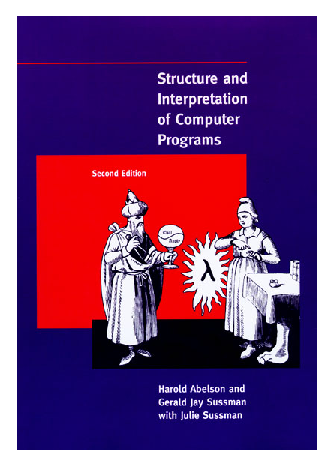
\includegraphics[width=20mm]{lecture0/SICP.eps}
          \caption{Харольд Абельсон, Джеральд Джей Сассман ``Структура и интерпретация компьютерных программ''}
      \end{center}
    \end{minipage}
  \end{figure}
\end{frame}

\begin{frame}{Учебники}
  \begin{figure}[h]
    \begin{minipage}[h]{0.49\linewidth}
      \begin{center}
          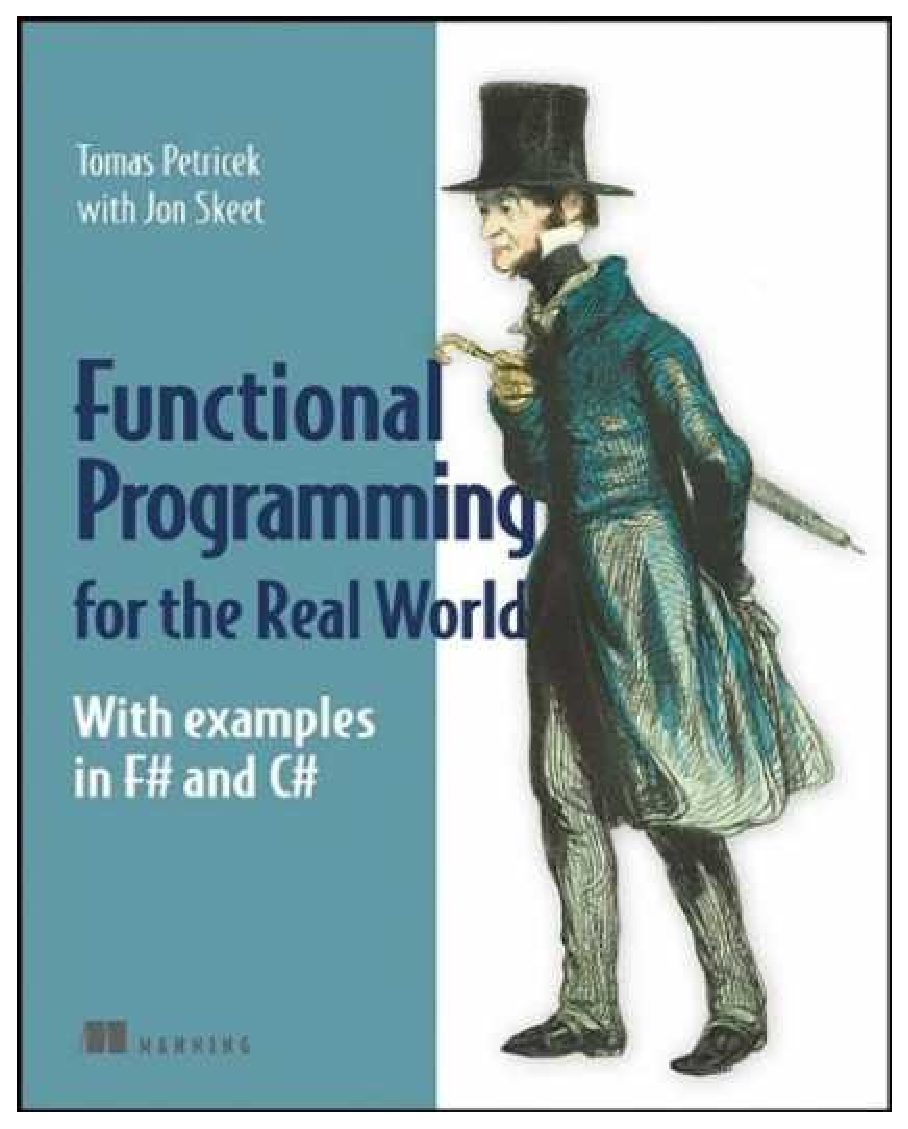
\includegraphics[width=20mm]{lecture0/FPiRW.eps}
          \caption{Томас Петричек, Джон Скит ``Functional Programming for the Real World''}
      \end{center}
    \end{minipage}
    \begin{minipage}[h]{0.49\linewidth}
      \begin{center}
        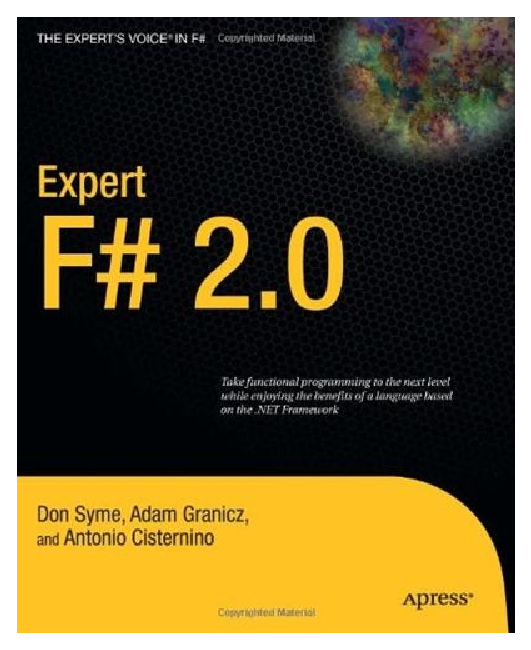
\includegraphics[width=20mm]{lecture0/Expert_Fsharp.eps}
        \caption{Дон Сайм ``Expert F\# 2.0''}
      \end{center}
    \end{minipage}
  \end{figure}
\end{frame}

\begin{frame}{Рекомендуемая литература}
  \begin{figure}
    \begin{minipage}{0.3\linewidth}
      \begin{center}
        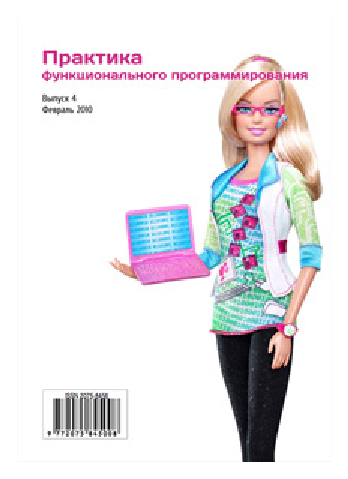
\includegraphics[width=20mm]{lecture0/pfp2010-04.eps}
      \end{center}
    \end{minipage}
    \begin{minipage}{0.3\linewidth}
      \begin{center}
        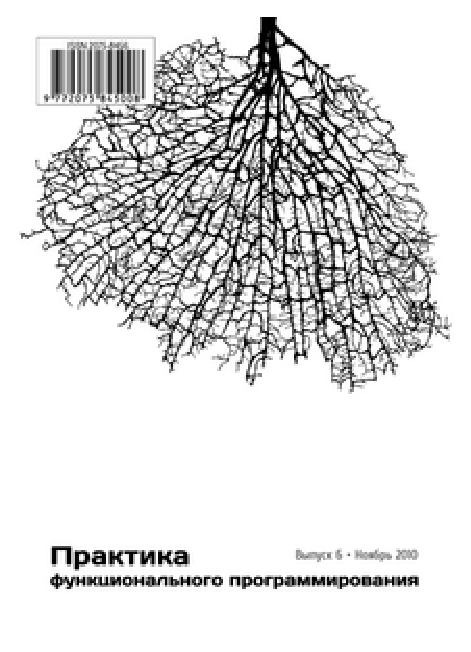
\includegraphics[width=20mm]{lecture0/pfp2010-06.eps}
      \end{center}
    \end{minipage}
    \begin{minipage}{0.3\linewidth}
      \begin{center}
        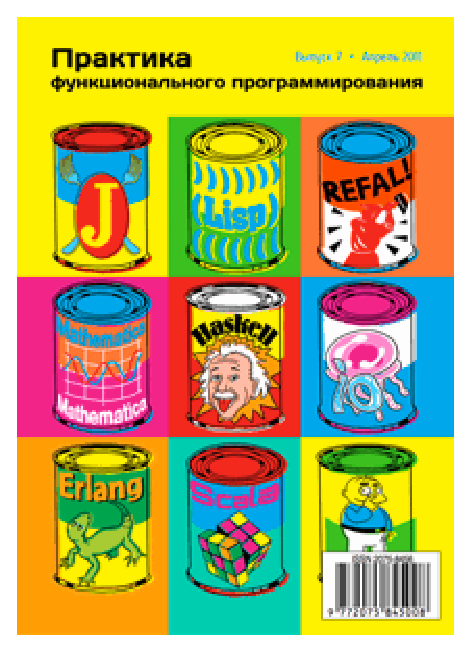
\includegraphics[width=20mm]{lecture0/pfp2011-07.eps}
      \end{center}
    \end{minipage}
    \caption{Журнал ``Практика функционального программирования''}
  \end{figure}
\end{frame}

\begin{frame}
  \begin{center}
    \LARGE{Вопросы?}
  \end{center}
\end{frame}

\end{document}
